\documentclass[handout, dvipsnames]{beamer}
\mode<presentation>{}
\usepackage[utf8]{inputenc}
\usepackage{amsmath, amssymb, amsfonts, amsthm, mathtools, mathrsfs}
\setbeamertemplate{theorems}[numbered]
\title{Galois correspondence in Algebraic Topology}
\author[Aryaman Maithani]{\texorpdfstring{Aryaman Maithani\\(Supervisor: Prof. Rekha Santhanam)}{Aryaman Maithani}}
\date[23-10-2020]{October 23, 2020}
\institute[IITB]{\texorpdfstring{Department of Mathematics\\IIT Bombay}{IIT Bombay}}
\usetheme{Warsaw}
\usepackage{parskip}
\usepackage{tcolorbox}
\usepackage{tikz-cd}
\tikzset{
    invisible/.style={opacity=0},
    visible on/.style={alt={#1{}{invisible}}},
    alt/.code args={<#1>#2#3}{%
      \alt<#1>{\pgfkeysalso{#2}}{\pgfkeysalso{#3}}%
  }
}
\setbeamercolor{footline}{fg=blue}
\setbeamerfont{footline}{series=\bfseries}
\addtobeamertemplate{navigation symbols}{}{%
    \usebeamerfont{footline}%
    \usebeamercolor[fg]{footline}%
    \hspace{1em}%
    \insertframenumber/\inserttotalframenumber
}
% \usepackage{tikz}
% \usecolortheme{beetle}
% \usepackage{graphicx}
\let\emptyset\varnothing

\newcommand{\id}{\operatorname{id}}
% \renewcommand{\exp}{\operatorname{exp}}

\theoremstyle{definition}
\newtheorem{defn}{Definition}
\newtheorem{thm}{Theorem}
\newtheorem{prop}[thm]{Proposition}
\newtheorem{cor}[thm]{Corollary}
\begin{document}
\begin{frame}
    \titlepage
\end{frame}
% \begin{frame}{Introduction}
%     We start with a definition of covering spaces.
% \end{frame}
\begin{frame}{Covering spaces}
    \begin{defn}[Covering spaces]
        \uncover<2->{$E\overset{p}{\longrightarrow}X$ is said to be a \emph{covering space} of $X$ }\uncover<3->{if every $x \in X$ }\uncover<4->{has an open neighbourhood $U$ }\uncover<5->{such that $p^{-1}(U)$ is a disjoint union of open sets $S_i$ in $E,$ }\uncover<6->{each of which is mapped homeomorphically onto $U$ by $p.$ }%\uncover<7->{Such $U$ are said to be \emph{evenly covered,} and the $S_i$ are called \emph{sheets} over $U.$ }
    \end{defn}
    \only<1>{\begin{center}
            
\includegraphics[width=7.5 cm]{covdef0.jpg}
    \end{center}}
    \only<2>{\begin{center}
            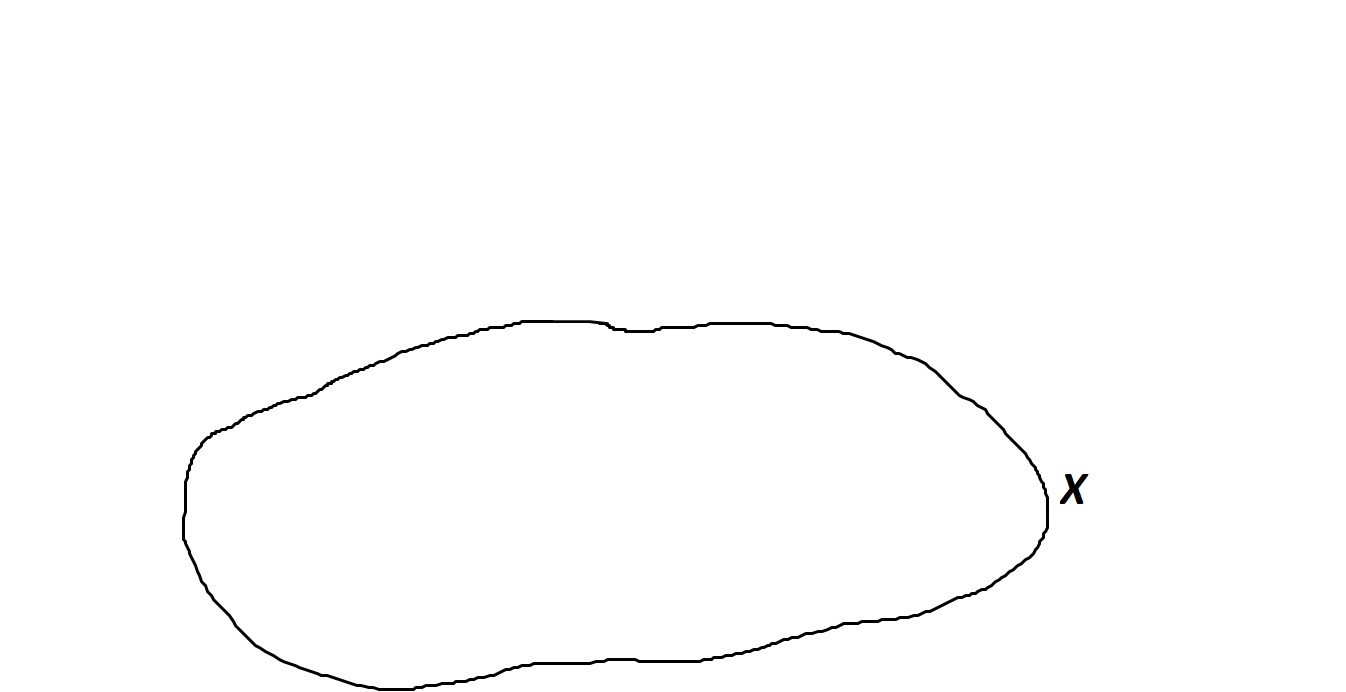
\includegraphics[width=7.5 cm]{covdef1.jpg}
    \end{center}}
    \only<3>{\begin{center}
            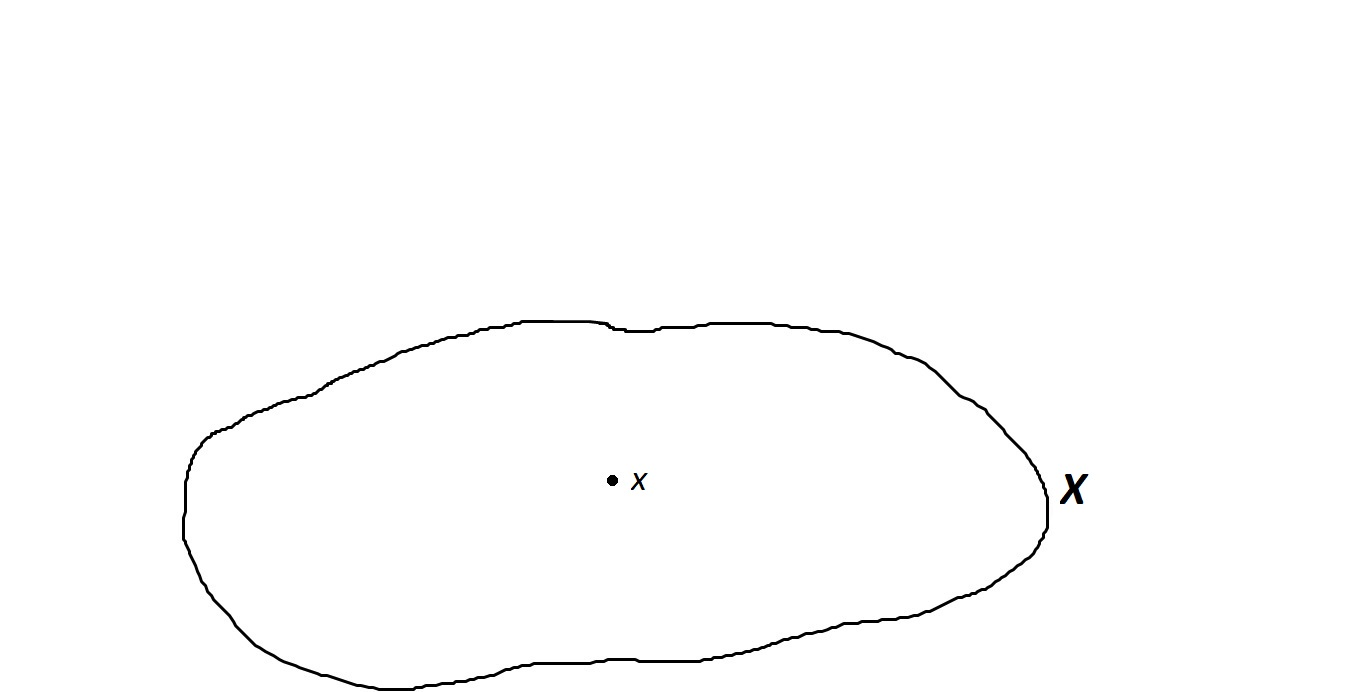
\includegraphics[width=7.5 cm]{covdef2.jpg}
    \end{center}}
    \only<4>{\begin{center}
            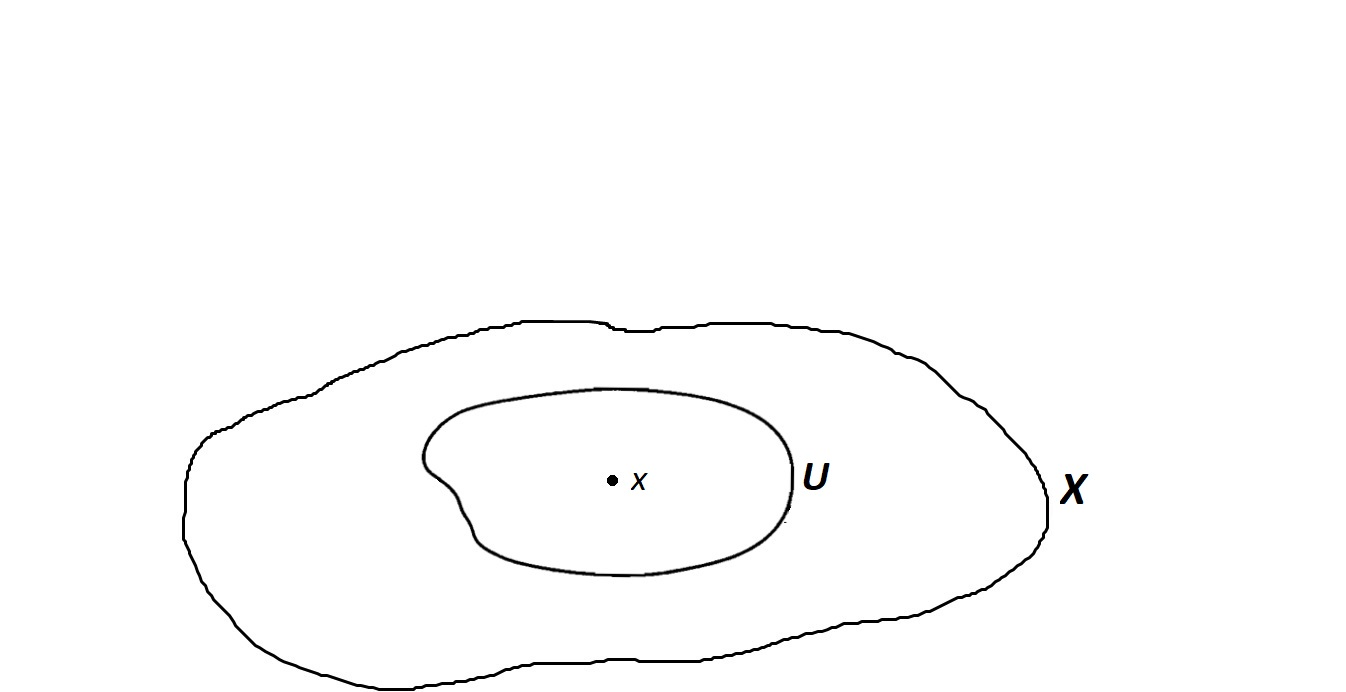
\includegraphics[width=7.5 cm]{covdef3.jpg}
    \end{center}}
    \only<5>{\begin{center}
            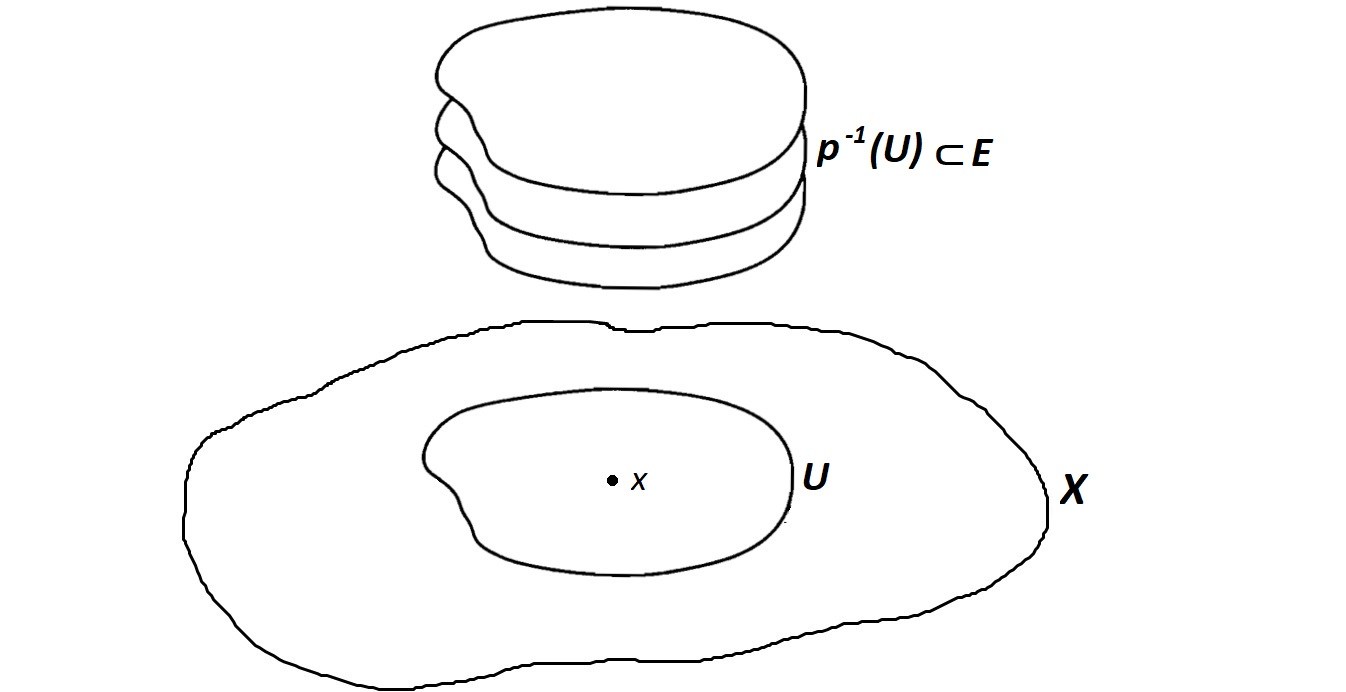
\includegraphics[width=7.5 cm]{covdef4.jpg}
    \end{center}}
    \only<6->{\begin{center}
            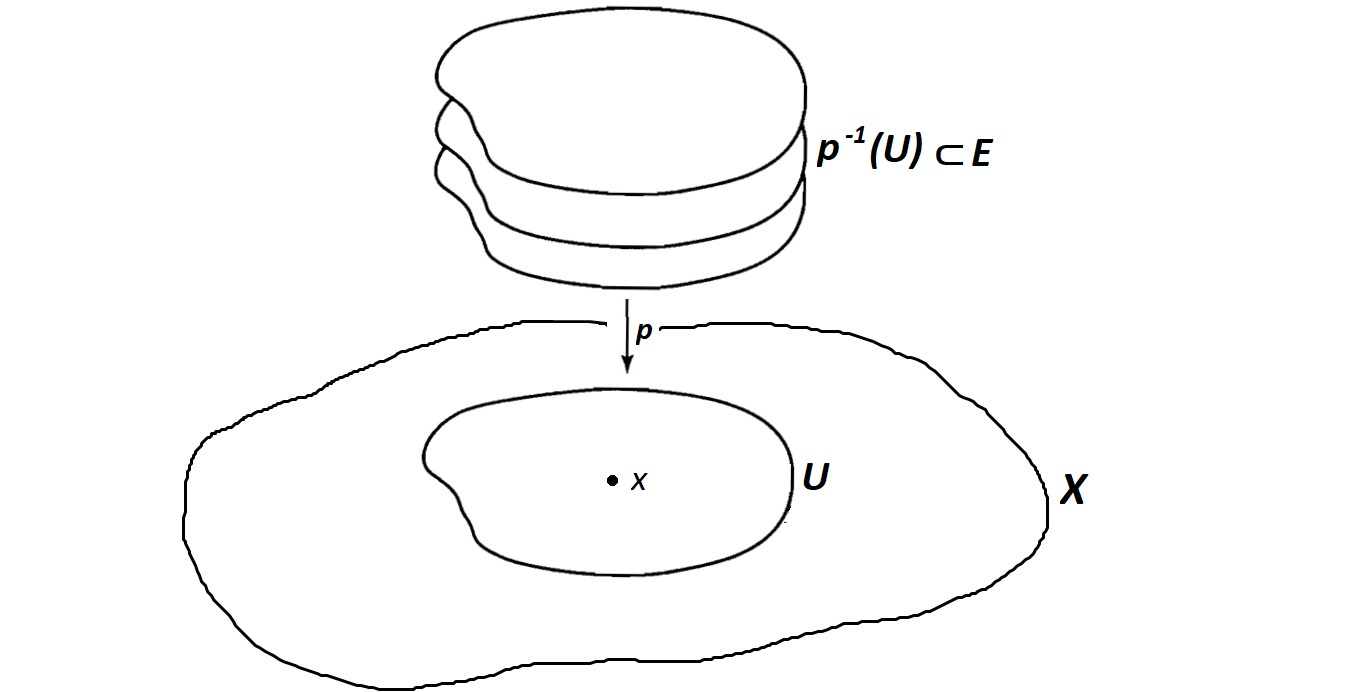
\includegraphics[width=7.5 cm]{covdef5.jpg}
    \end{center}}
\end{frame}
\begin{frame}{Examples}
    Let us take $X = S^1 \subset \mathbb{C}.$
    \begin{enumerate}
        \uncover<2->{\item Take $E = \mathbb{R}$ and $p : \mathbb{R} \to S^1$ defined by }\uncover<3->{$x \mapsto e^{2\pi\iota x}.$ }
        \uncover<4->{\begin{center}
        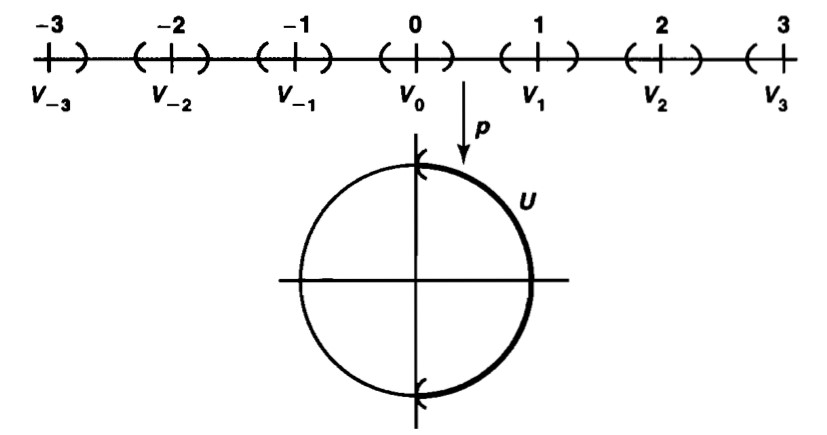
\includegraphics[width=7.5 cm]{R-covering-S1.jpg}
        \end{center} }
        \uncover<5->{\item $E' = S^1$ and $p_n:S^1 \to S^1$ defined by }\uncover<6->{$z \mapsto z^n.$ }
    \end{enumerate}
    % \uncover<7->{In fact, a covering map is a quotient map, in general. }
\end{frame}
\begin{frame}{Group of covering transformations}
    \begin{defn}[Group of covering transformations]
        \uncover<2->{Given a covering space $E \overset{p}{\longrightarrow} X,$ }\uncover<3->{the group $G$ of \emph{covering transformations} is the group }\uncover<4->{of all homeomorphisms of $E$ which preserves the fibers, }\uncover<5->{that is, all those $\varphi$ such that $p\varphi = p.$ }
    \end{defn}
    \uncover<6->{Said differently, it is the group of all homeomorphic lifts of $p.$ }
    \uncover<2->{\begin{center}
            \begin{tikzcd}[ampersand replacement=\&]
                {E} \arrow[visible on=<5->, rr, "\varphi"]\arrow[rdd, "p"'] \&\& {E} \arrow[ldd, "p"]\\
                \&\&\\
                \& X \&
            \end{tikzcd}
        \end{center} }
\end{frame}
\begin{frame}{Examples}
    Let us look at the group of covering transformations for the earlier examples.
    \begin{enumerate}
        \uncover<2->{\item $\mathbb{R}\overset{p}{\longrightarrow}S^1$ 

        The desired homeomorphisms are precisely those of the form }\uncover<3->{$x \mapsto x+n$ for $n \in \mathbb{Z}.$ }\uncover<4->{Thus, $G \cong \mathbb{Z}$ here. }
        \uncover<5->{\item $S^1 \overset{p_n}{\longrightarrow} S^1$}

        \uncover<6->{The desired homeomorphisms are precisely multiplication by $n$-th roots of unity. }\uncover<7->{Thus, $G \cong \mathbb{Z}/n\mathbb{Z}$ here. }
    \end{enumerate}
\end{frame}
\begin{frame}{Disclaimer and Definitions}
    \begin{tcolorbox}
        We shall now assume that all spaces are locally path-connected and path-connected.
    \end{tcolorbox}
    \uncover<2->{\begin{tcolorbox}
        Recall that given a map $E\overset{p}{\longrightarrow}X,$ we get a homomorphism $p_*:\pi_1(E, e_0) \to \pi_1(X, p(e_0))$ \uncover<3->{as $[\tau] \mapsto [p\circ\tau].$ }
        \end{tcolorbox} 
    }
    \uncover<4->{\begin{tcolorbox}
    A \emph{map} between topological spaces is a continuous function between them. \\
    \uncover<5->{A map of the form $f:(X, x_0) \to (Y, y_0)$ is a continuous function $f:X\to Y$ such that $f(x_0) = y_0.$ }
    \end{tcolorbox}}
\end{frame}
\begin{frame}{Lifting criterion}
    \begin{thm}[The lifting criterion]
        \uncover<2->{Consider the situation 
        \begin{center}
            \begin{tikzcd}[ampersand replacement=\&]
                {(Y, y_0)} \arrow[dddrr, "f"']\arrow[visible on=<4->, rr, "f'", dashed] \& \& {(E, e_0)} \arrow[ddd, "p"]\\
                \& \& \\
                \& \& \\
                \& \& {(X, x_0)} 
            \end{tikzcd}
        \end{center} }
        \uncover<3->{where $p$ is a covering map and $f$ an arbitrary map. }\uncover<5->{The lift $f'$ exists if and only if }\uncover<6->{
        \begin{equation*} 
            f_*\pi_1(Y, y_0) \subset p_*\pi_1(E, e_0).
        \end{equation*} }
        \uncover<7->{In such a case, the lift is {\color{Sepia}\underline{unique}}. }
    \end{thm}
\end{frame} 
\begin{frame}{Lifting criterion}
    \uncover<2->{\begin{cor}
        If $Y$ is simply connected, \uncover<3->{the lift $f'$ exists. }
    \end{cor} }
    \uncover<4->{
    \begin{prop}
        If $Y \overset{f}{\longrightarrow} X$ is also a covering space, and $f'$ exists, \uncover<5->{then $Y \overset{f'}{\longrightarrow} E$ is a covering space.  }
    \end{prop} }
    \uncover<6->{Thus, we get a diagram\ }\uncover<7->{{\color{blue}\begin{tikzcd}
        {(Y, y_0)} \arrow[dd, "f'"] \\
                                                                   \\
        {(E, e_0)} \arrow[dd, "p"]                                 \\
                                                                   \\
        {(X, x_0)}                                                
        \end{tikzcd}} }\uncover<8->{\ of covering spaces. }
         
\end{frame}
\begin{frame}{Equivalent covering spaces}
    \begin{cor}
        \uncover<2->{If $(E, e_0) \overset{p}{\longrightarrow} (X, x_0)$ }\uncover<3->{and $(E', e_0') \overset{p'}{\longrightarrow} (X, x_0)$ are covering spaces of $X$} \uncover<4->{such that $p_*\pi_1(E, e_0) = p'_*\pi_1(E', e_0'),$ }\uncover<5->{then there is a {\color{Sepia}\underline{unique}} homeomorphism
            \begin{equation*} 
                \varphi:(E, e_0) \to (E', e_0')
            \end{equation*} }
        \uncover<5->{such that $p'\varphi = p.$ }
    \end{cor}
    \uncover<6->{In such a case, we call the coverings \emph{equivalent.} }
    \uncover<2->{\begin{center}
            \begin{tikzcd}[ampersand replacement=\&]
                {(E, e_0)} \arrow[visible on=<5->, rr, "\varphi"]\arrow[rdd, "p"'] \&\& |[visible on=<3->]|{(E', e_0')} \arrow[visible on=<3->, ldd, "p'"]\\
                \&\&\\
                \& {(X, x_0)} \&
            \end{tikzcd}
        \end{center} }
\end{frame}
\begin{frame}{Equivalent covering spaces: Proof}
    \emph{Proof.} \uncover<3->{Since $p_*\pi_1(E, e_0) = p'_*\pi_1(E', e_0'),$ the lifts shown exist. }
    \uncover<2->{
    \begin{center}
    \begin{tikzcd}[ampersand replacement=\&]
        {(E, e_0)} \arrow[rdd, "p"'] \arrow[visible on=<3->, rr, "\varphi", bend left=10] \arrow[visible on=<4->, "\id_E"', loop, distance=2em, in=215, out=145] \&\& {(E', e_0')} \arrow[ldd, "p'"] \arrow[visible on=<3->, ll, "\varphi'", bend left=10] \arrow[visible on=<4->, "\id_{E'}"', loop, distance=2em, in=35, out=325] \\
        \&\&\\
        \&{(X, x_0)} \& 
    \end{tikzcd} 
    \end{center} }

    \uncover<5->{{\color{Sepia}\underline{Unique}}ness forces $\varphi\circ\varphi'$ and $\varphi'\circ\varphi$ to be the identity maps. }\uncover<6->{Thus, $\varphi$ is an homeomorphism proving the equivalence. }

    \uncover<7->{Note that we actually showed that any two $\varphi$ and $\varphi'$ as pictured must be inverses of each other. }\uncover<8->{In particular, $\varphi$ is {\color{Sepia}\underline{unique}.} }\uncover<9->{\hfill $\qed$}
\end{frame}
\begin{frame}{Universal covering space} 
    \uncover<2->{If $(X, x_0)$ has a covering space $(\tilde{X}, \widetilde{x_0}) \to (X, x_0)$ such that $\tilde{X}$ is simply connected, }\uncover<3->{then $(\tilde{X}, \widetilde{x_0})$ is unique up to equivalence. }
    \uncover<4->{\begin{defn}[Universal covering]

        \uncover<4->{We call such a covering space ``the'' \emph{universal covering space} of $(X, x_0).$ }
    \end{defn} }

    \uncover<5->{$\tilde{X}$ is \emph{universal} in the sense that every other covering space is {\color{blue}\emph{below}} it; it covers every other covering space. }

    \uncover<6->{
    \begin{tcolorbox}
        Does every space have a universal covering space?
    \end{tcolorbox} }
\end{frame}
\begin{frame}{Universal covering space}
    % \begin{defn}[Semi-locally simply connected]
    %     \uncover<2->{A space $X$ is called \emph{semi-locally simply connected} if it has the following property:\\ }
    %     \uncover<3->{For any $x \in X,$ there is a neighborhood $U$ }\uncover<4->{such that any loop in $U$ based at $x$ }\uncover<5->{can be shrunk {\color<6->{red}in $X$} to $x.$ }\uncover<7->{(In the process of shrinking the loop, we may go outside of $U.$) }
    % \end{defn}
    \uncover<1->{Well, note that a covering map is a local homeomorphism. }\uncover<2->{Thus, small enough loops in $X$ can be lifted to \emph{loops} in $\tilde{X}.$ }\uncover<3->{Thus, these loops must be shrinkable to a point. }\uncover<4->{This gives us a necessary condition. }\uncover<5->{The space must be \emph{semi-locally simply connected}. }\uncover<6->{In fact, this is sufficient as well! }

    \uncover<6->{\begin{thm}[Existence of universal covering space]
        \uncover<7->{If $X$ is a semi-locally simply connected space, }\uncover<8->{then $X$ has a universal covering. }
    \end{thm} }
\end{frame}
\begin{frame}{Lifting paths}
    The lifting criterion also shows that paths in $X$ can always be lifted to paths in $E.$ \uncover<2->{This is because $[0, 1]$ is simply connected. }\uncover<3->{Moreover, we can choose any point in $p^{-1}(x_0)$ to be the starting point. }

    \uncover<4->{In fact, more is true. One can lift path homotopies as well. }%\uncover<5->{(The point being that the lift is still a path homotopy between the lifts of the paths.) }

    \uncover<5->{Thus, if two loops are homotopic in $X,$ then their lifts are homotopic as well. }\uncover<6->{In particular, they have the same endpoint. }

    % \uncover<8->{This also shows that $p_*:\pi_1(E, e_0) \to \pi_1(X, x_0)$ is injective. }
\end{frame}
\begin{frame}{Computation of fundamental group}
    \uncover<1->{\begin{thm}   
        \uncover<2->{Let $(E, e_0) \overset{p}{\longrightarrow} (X, x_0)$ be a covering space with group of covering transformations $G.$ }\uncover<3->{If $E$ is simply connected, }\uncover<4->{then $\pi_1(X, x_0)\cong G.$ }
    \end{thm} }
    \begin{proof}[Sketch]
    \uncover<5->{The isomorphism ${\color{ForestGreen}\Phi}:\pi_1(X, x_0) \to G$ is given as follows: }\\~\\
    %
    \uncover<6->{Given $[\sigma] \in \pi_1(X, x_0),$ }\uncover<7->{pick a lift $\tilde{\sigma}:[0, 1] \to E$ }\uncover<8->{with $\tilde{\sigma}(0) = e_0.$ }\\~\\
    %
    \uncover<9->{Set $e_1 \vcentcolon= \tilde{\sigma}(1).$ }\uncover<10->{Then, there exists a unique $g \in G$ with $g(e_0) = e_1.$ }\\~\\
    %
    \uncover<11->{The map $[\sigma] \mapsto g$ is well-defined and an isomorphism. }
    \end{proof}
    % \uncover<12->{That it is a bijection is easy to check by constructing an inverse. }\uncover<13->{It being a homomorphism is also not too tough and just involves chasing the definitions. }
\end{frame}
\begin{frame}{Computation of covering spaces}
    \begin{cor}
        $\pi_1(S^1, 1+0\iota) \cong \mathbb{Z}.$
    \end{cor}
    \uncover<2->{\begin{proof} 
        The covering map $\mathbb{R}\overset{p}{\longrightarrow}S^1$ seen earlier had $G \cong \mathbb{Z}$ \uncover<3->{and $\mathbb{R}$ is simply connected. }
    \end{proof} }
\end{frame}
    
% \begin{frame}{Computation of fundamental group}
%     \uncover<1->{\begin{thm}
%         If we don't assume $E$ to be simply connected, we have \uncover<2->{
%         \begin{equation*} 
%             G \cong N/p_*\pi_1(E, e_0),
%         \end{equation*} }\uncover<3->{where $N$ is the normaliser of $p_*\pi_1(E, e_0)$ in $\pi_1(X, x_0).$ }
%     \end{thm} }
% \end{frame}

% \begin{frame}{Universal covering space}
%     \begin{thm}
%         \uncover<2->{If $(E, e_0) \overset{p}{\longrightarrow} (X, x_0)$ }\uncover<3->{and $(E', e_0') \overset{p'}{\longrightarrow} (X, x_0)$ are both simply-connected covering spaces of $X,$} \uncover<4->{then there is a unique homeomorphism
%             \begin{equation*} 
%                 \varphi:(E, e_0) \to (E', e_0')
%             \end{equation*} }
%         \uncover<4->{such that $p'\varphi = p.$ }
%     \end{thm}
%     \uncover<5->{In such a case, we call the coverings \emph{equivalent.} }
%     \uncover<2->{\begin{center}
%             \begin{tikzcd}[ampersand replacement=\&]
%                 {(E, e_0)} \arrow[visible on=<4->, rr, "\varphi"]\arrow[rdd, "p"'] \&\& |[visible on=<3->]|{(E', e_0')} \arrow[visible on=<3->, ldd, "p'"]\\
%                 \&\&\\
%                 \& {(X, x_0)} \&
%             \end{tikzcd}
%         \end{center} }
% \end{frame}
\begin{frame}{Even actions}
    Now, we do something in the opposite direction. \uncover<2->{We start with a topological space $E$ and }\uncover<3->{{\color{red}a} group $G$ of homeomorphisms of $E.$ }\uncover<4->{From this, we construct a covering space. }

    \uncover<5->{\begin{defn}[Even action]
        Let $G$ be a group of homeomorphisms of $E.$ \uncover<6->{$G$ is said to act evenly on $E$ if for every $e \in E,$ }\uncover<7->{there exists a neighbourhood $U$ of $E$ }\uncover<8->{such that $U\cap gU = \emptyset$ }\uncover<9->{for all $1 \neq g \in G.$ }
    \end{defn} }

    \only<1-4>{\begin{center}
            
\includegraphics[width=7.5 cm]{evenact0.jpg}
    \end{center}}
    \only<5>{\begin{center}
            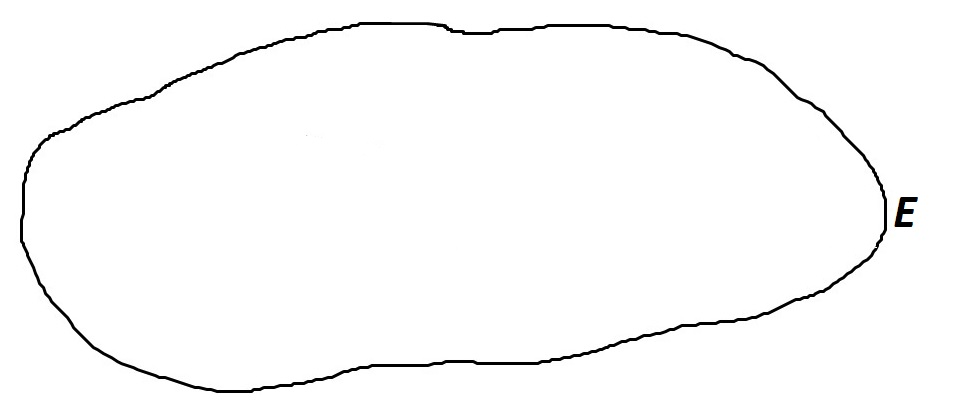
\includegraphics[width=7.5 cm]{evenact1.jpg}
    \end{center}}
    \only<6>{\begin{center}
            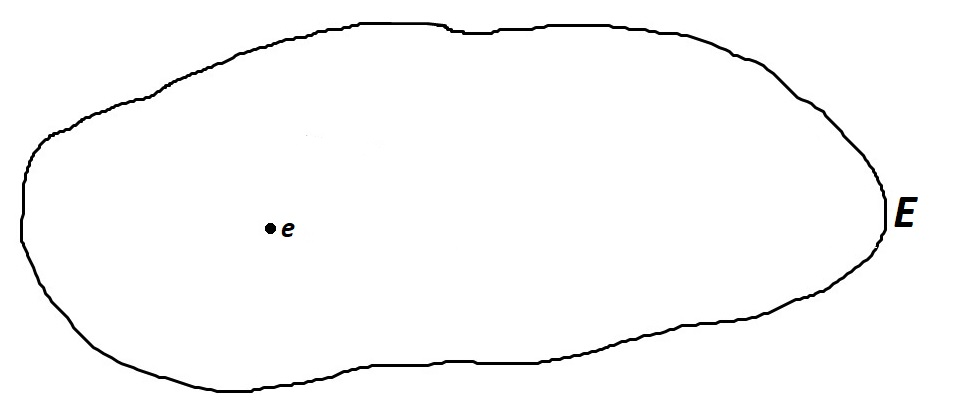
\includegraphics[width=7.5 cm]{evenact2.jpg}
    \end{center}}
    \only<7>{\begin{center}
            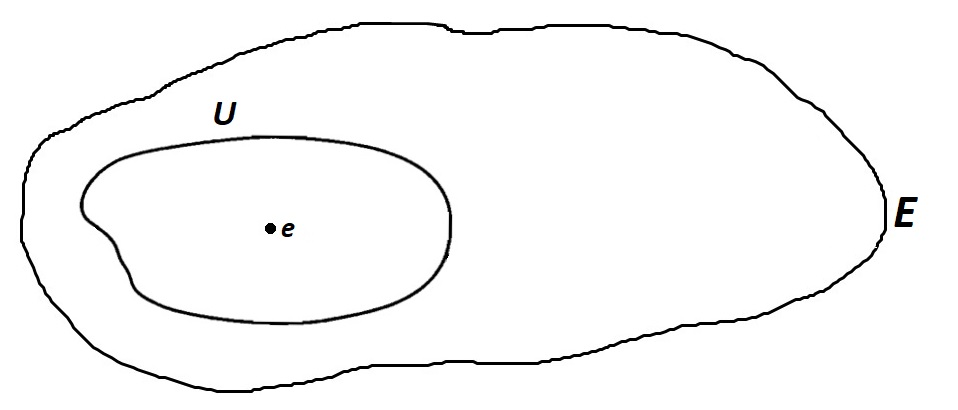
\includegraphics[width=7.5 cm]{evenact3.jpg}
    \end{center}}
    \only<8-9>{\begin{center}
            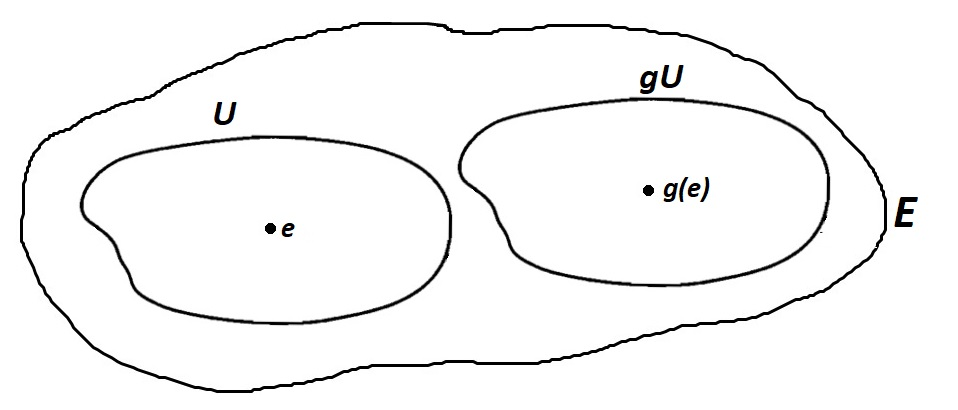
\includegraphics[width=7.5 cm]{evenact4.jpg}
    \end{center}}

    \only<10->{
    \uncover<10->{Given such a group, define $X = E/G$ to be the space of orbits. }\uncover<11->{Define $\pi:E \to X$ as the quotient map $e \mapsto Ge.$ }
    
    \uncover<12->{Then, $E\overset{\pi}{\longrightarrow}X$ is a covering space, and }
    \uncover<13->{\\ $G$ is its group of covering transformations.} }%, }\\
    %\uncover<14->{$p_*\pi_1(E, e_0)$ is a normal subgroup of $\pi_1(X, p(e_0))$ for all $e_0 \in E.$ }
\end{frame}
\begin{frame}{Even actions}
    If $(\tilde{X}, \widetilde{x_0}) \overset{p}{\longrightarrow} (X, x_0)$ is a covering space \uncover<2->{with $\tilde{X}$ simply connected }\uncover<3->{and $G$ its group of covering transformations, }\uncover<4->{then $G$ acts evenly on $E.$ }

    \uncover<5->{Moreover, $\tilde{X}/G$ is homeomorphic to $X.$ }\uncover<6->{This homeomorphism is the natural one as shown in the following diagram. }

    \uncover<7->{\begin{center}
            \begin{tikzcd}[ampersand replacement=\&]
                {\tilde{X}} \arrow[dd, "\pi"']\arrow[rrdd, "p"] \& \& \\
                \& \& \\
                {\tilde{X}/G}\arrow[visible on=<8->, rr, "\cong"'] \& \& {X}
            \end{tikzcd}
        \end{center} }

    \uncover<9->{To summarise: we can recover $X$ (up to homeomorphism) from $\tilde{X}$ and $G.$ }
\end{frame}
\begin{frame}{Galois correspondence}
    \begin{thm}[Galois correspondence]
        \uncover<2->{Let $(X, x_0)$ be a (pointed) topological space with a universal covering space. }\uncover<3->{Let $H$ be a subgroup of $\pi_1(X, x_0).$ }\uncover<4->{Then, there exists a covering space $(E, e_0) \overset{p}{\longrightarrow} (X, x_0)$ unique up to equivalence such that }\uncover<5->{
            \begin{equation*} 
                p_*\pi_1(E, e_0) = H.
            \end{equation*} }
        \uncover<6->{Thus, there is a one-one correspondence between the covering spaces of $X$ and subgroups of $\pi_1(X, x_0).$ }
    \end{thm}
    \uncover<7->{In the example of $X = S^1,$ }\uncover<8->{$\mathbb{R}$ is the universal covering space corresponding to $\langle 0\rangle.$ }\uncover<9->{For a nontrivial subgroup $n\mathbb{Z},$ }\uncover<10->{we have $E = S^1$ and the map $z \mapsto z^n.$ }
\end{frame}
\begin{frame}{Galois correspondence: Proof}
    \textbf{Existence.} \uncover<2->{Let $(\tilde{X}, \widetilde{x_0})$ be the universal covering space. }\uncover<3->{Let $G$ be the group of covering transformations.}\\
    \uncover<4->{Recall the isomorphism ${\color{ForestGreen}\Phi}:\pi_1(X, x_0) \to G.$ }\uncover<5->{Let $H' = {\color{ForestGreen}\Phi}(H).$ }\uncover<6->{$H'$ acts evenly on $\tilde{X}.$ }

    \uncover<7->{Consider $(E, e_0) \vcentcolon= (\tilde{X}/H', H'\widetilde{x_0}).$ }\uncover<9->{Now, we get an induced covering map $p$ as follows. }

    \uncover<8->{\begin{center}
        \begin{tikzcd}[ampersand replacement=\&]
            {(\tilde{X}, \widetilde{x_0})} \arrow[dd, "\pi"'] \arrow[rrdd, "q"] \& \&\\
            \&  \&\\
            {(E, e_0)} \arrow[visible on=<10->, rr, "p"'] \& \& {(X, x_0)}
        \end{tikzcd}
    \end{center} }
\end{frame}
% \begin{frame}{Galois correspondence: Proof (contd.)}
%     We now show that $p_*\pi_1(E, e_0) = H.$

%     \uncover<2->{$(\supset)$} \uncover<3->{Let $[\sigma] \in H.$ }\uncover<4->{${\color{ForestGreen}\Phi}([\sigma]) \in H'.$ }

%     \uncover<5->{Let $\tilde{\sigma}$ be a lift to $\tilde{X}$ with $\tilde{\sigma}(0) = \widetilde{x_0}.$ }\uncover<6->{Put $\widetilde{x_1} \vcentcolon= \tilde{\sigma}(1).$ }

%     \uncover<7->{Then, there is a homeomorphism $h \in H'$ such that $h(\widetilde{x_0}) = \widetilde{x_1}.$ }\uncover<8->{Thus, $H'\widetilde{x_0} = H'\widetilde{x_1}$ and hence, $\pi\circ\tilde{\sigma}$ is a loop. }\uncover<9->{But we have $p\circ\pi\circ\tilde{\sigma} = q\circ\tilde{\sigma} = \sigma.$ }

%     \uncover<10->{Thus, $[\sigma] = p_*([\pi\circ\tilde{\sigma}]) \in p_*\pi_1(E, e_0).$ }
% \end{frame}
% \begin{frame}{Galois correspondence: Proof (contd.)}
%     $(\subset)$ \uncover<2->{Consider a loop $\tau$ in $E$ at $e_0.$ }\uncover<3->{We wish to show $[p\circ\tau] \in H.$ }

%     \uncover<4->{Let $\sigma = p\circ\tau.$ }\uncover<5->{This is a loop in $X$ at $x_0.$ Consider a lift $\tilde{\sigma}$ in $\tilde{X}$ with $\tilde{\sigma}(0) = \widetilde{x_0}.$ }

%     \uncover<6->{Now, note that $\tau = \pi\circ\tilde{\sigma}$ is a loop in $E.$ }\uncover<7->{Thus, $\pi(\widetilde{x_0}) = \pi(\widetilde{x_1}).$ }\uncover<8->{This tells us that $H'\widetilde{x_0} = H'\widetilde{x_1}.$ }

%     \uncover<9->{In other words, there exists $h \in H'$ such that $h(\widetilde{x_0}) = \widetilde{x_1}.$ }\uncover<10->{Thus, ${\color{ForestGreen}\Phi}([\sigma]) \in H'$ or $[\sigma] \in H,$ }\uncover<11->{as desired. }\hfill\uncover<12->{$\qed$ }
% \end{frame}
\begin{frame}{Galois correspondence: Proof (contd.)}
    \uncover<2->{We now show that $p_*\pi_1(E, e_0) = H.$ }

    \uncover<3->{Let $[\sigma]$ be an arbitrary element of $\pi_1(X, x_0).$ } 

    \uncover<4->{Consider the lift $\tilde{\sigma}$ in $\tilde{X}$ with $\tilde{\sigma}(0) = \widetilde{x_0}.$ }\uncover<5->{Put $\widetilde{x_1} \vcentcolon= \tilde{\sigma}(1).$ }

    \uncover<6->{Let $\tau = \pi\circ\tilde{\sigma}.$ }\uncover<7->{This is a path in $E$ starting at $e_0.$ }\uncover<8->{Moreover, it is the unique lift of $\sigma$ starting at $e_0.$ } \\
    \uncover<9->{Thus, if $\tau$ is a loop, then $[\sigma] = p_*([\tau]) \in p_*\pi_1(E, e_0).$ } \\
    \uncover<10->{More importantly, if $\tau$ is \emph{not} a loop, }\uncover<11->{then $[\sigma] \notin p_*\pi_1(E, e_0).$ }

    \uncover<12->{Thus, $[\sigma] \in p_*\pi_1(E, e_0)$ iff $\tau$ is a loop. }

    \uncover<13->{Note that $\tau$ is a loop }\uncover<14->{iff $\pi(\widetilde{x_0}) = \pi(\widetilde{x_1})$ }\uncover<15->{iff there is a homeomorphism $h \in H'$ such that $h(\widetilde{x_0}) = \widetilde{x_1}$ }\uncover<16->{iff ${\color{ForestGreen}\Phi}([\sigma]) \in H'$ }\uncover<17->{iff $[\sigma] \in H.$ }

    \uncover<18->{Thus, $[\sigma] \in H \iff [\sigma] \in p_*\pi_1(E, e_0).$ }\hfill\uncover<19->{$\qed$ }
\end{frame}
\end{document}